%!TEX root = ../template.tex
%%%%%%%%%%%%%%%%%%%%%%%%%%%%%%%%%%%%%%%%%%%%%%%%%%%%%%%%%%%%%%%%%%%%
%% chapter10.tex
%% NOVA thesis document file
%%
%% Chapter with lots of dummy text
%%%%%%%%%%%%%%%%%%%%%%%%%%%%%%%%%%%%%%%%%%%%%%%%%%%%%%%%%%%%%%%%%%%%

\typeout{NT FILE chapter10.tex}%

\chapter{Conclusion and Future Work}
\label{cha:Conclusion}

In this work, fundamental topics in time series data mining were researched. These topics were motivation by considering the need for tools that help analysts to better understand what happened during the recording process and find relevant instances on signals that can be related with specific occurrences in the physical world. These motivations are intrinsically related with tools that are more visually interpretable and search mechanisms that are more expressive and intuitive. The work developed contributed to each of these domains with relevant standard mechanisms that can be further developed into practical tools for real scenarios. Not only these tool can be practical, but the methods presented bring novelty into the state of the art, either by "borrowing" more traditional methods from other domains (such as the \gls{ssm} in audio information retrieval or \gls{nlp} techniques for text mining) or by introducing novel concepts, specially in terms of text representation of biosignals and text-based query search mechanisms.
\par
In this Chapter, we highlight the main contributions of this thesis in each of this domains. Comments are also given regarding the contributions and applicability to occupational health scenarios. Finally, overall scientific production and collaborations during the period of this thesis are also provided. 

\section{Main Contributions on General Topics}

As we mentioned in Chapter \ref{cha:introduction}, this thesis contributes to three main topics, namely \textit{Sensing}, \textit{Analysis} and \textit{Decision Making}:
\begin{itemize}
\item \textit{Sensing:} In this context, a deep understanding of the existing technology to record biosignals was made. At some point, the focus moved towards technology existing to monitor occupational variables. A written work is available regarding the usage of fiber-optics for the monitoring of motion and postural variables in automotive industries, which can be found in \cite{fiber_optics} and it is compared to other existing methods. In addition, a study of the state of the art sensors existing on the market was made to understand the fit in the occupational health problematic. A presentation is available at \cite{sensors_slides}, showing the existing materials on the market and that cover human motion and physiology, more focused for occupational health. The contributions in this area are more related with the knowledge gained and how it was used to more appropriately prepare an acquisition plan regarding the acquisition of occupational variables in several settings, namely automotive industry (Volkswagen Autoeuropa), clothing manufacturers and office/desk jobs.\\

\item \textit{Analysis:} This work has demonstrated a deeper exploration of the topics related with the analysis of biosignals and time series in general. The contributions include the usage of the \gls{ssm} for the segmentation of time series (\textit{novelty} and \textit{periodic} functions), summarization and creation of similarity profiles for (semi-)automatic clustering. A novel symbolic representation of time series was introduced, and examples were provided in how to apply it for pattern search with \gls{regex} (\gls{ssts}) and text-based classification (\gls{hearts}). A novel search mechanism was also developed, closer to natural language search, with keywords and operators (\gls{quots}). A more detailed explanation of these contributions are provided on a further section.\\

\item \textit{Decision Making:} The main purpose of the studied and developed methods was to help analysts when inspecting time series, but also move towards democratizing pattern search on time series. The proposed strategies provide several levels of understanding and help in several layers of decision making. Of course it will depend on the purpose, context, output delivered by the method and the category of expertise of the analyst.
\par
Starting with the analysis of structural information with the \gls{ssm}, it provides a visual output that has characteristic structures that will appear independently of the type of data or context. The main information available on the \gls{ssm} will always be \textit{blocks}, \textit{paths} and \textit{similarity}. As we have seen, these can help the analyst identify specific occurrences on time series, with special interest in biosignals applications. Therefore, by learning how to retrieve information from the \gls{ssm}, more awareness is given to the analyst and more conscious decisions can be made based on that information.
\par
From a standard perspective, the analyst can also perform automatic or semi-automatic segmentation and labeling/annotation of data to accelerate the preparation process to train supervised machine learning algorithms. This can either be done with the visual support of the \gls{ssm} or the methods developed to extract the information automatically.
\par
Regarding the process of pattern search with more expressive queries, we believe the tools provide valuable resources to both the analyst that works in the time series domain and is experienced in the computer science field (e.g. a researcher that develops machine learning methods for biosignals processing), and the analyst that is not an expert in computer science but has knowledge in a specific domain of time series (e.g. a physician that is experienced in \gls{ecg} data). In this case, the process is more interactive and requires writing a \gls{regex}/text query. This should be useful to accelerate the search process by an experience computer scientist, because it should be more quick to make the search with this system than developing an algorithm for that purpose. In addition, it contributes to democratize the search mechanism to more analysts than only computer scientists, because if the analyst is able to describe the shape being searched, it should be possible to find it (considering the right connotation methods/word feature vectors are used). In that aspect, the information retrieval would quickly help the analyst in taking more informed decisions.
\end{itemize}


\section{Scientific Contributions}

\subsection{Unveiling the \textit{Grammar} of Time Series}

One of the major topics of this work regarded the segmentation of time series into smaller segments, based on \textit{novelty} and \textit{periodicity}. In addition, it was also discussed the benefit of relating the resulting subsequences by how similar these are. As an example, we showed the \gls{abp} signal \vstretch{0.6}{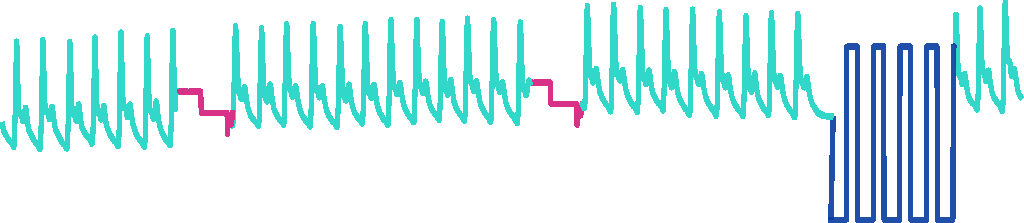
\includegraphics[width=25ex, valign=m]{bvp_thumbnail_final.pdf}}, which can be divided into 7 segments, having the structure \textcolor{mygreen3}{A} \textcolor{mymagenta}{B} \textcolor{mygreen3}{A} \textcolor{mymagenta}{B} \textcolor{mygreen3}{A} \textcolor{myblue5}{C} \textcolor{mygreen3}{A}. We demonstrated with strong evidences that the usage of the \gls{ssm} is reliable in performing this type of task. From the \gls{ssm}, the novelty function can be extracted and the similarity profiles can be compared to perform a segmentation and association between subsequences. In addition, the segmentation might be periodic, meaning that a signal, such as 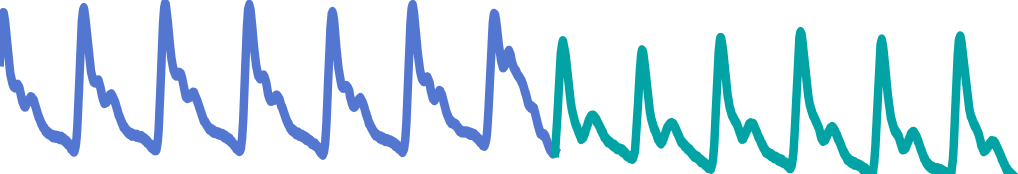
\includegraphics[height=2.5ex, valign=m]{bvpABpng.png}, can be separated into \textcolor{myblue}{A} and \textcolor{mygreen}{B}, but also, \textcolor{myblue}{AAAAAAA}\textcolor{mygreen}{BBBBBB}. We also demonstrated that using the \gls{ssm}, we can compute the similarity function, which highlights the cyclic nature of the subsequence.
\par
The performance of the method was validated for the novelty segmentation  process. It was compared to several SOA methods, showing to be competitive in tasks related with change point detection and segmentation. In addition, several use-cases from various fields were presented as examples, showing that the algorithm is agnostic to the type of signal, applicable to multidimensional and multimodal signals, and not requiring any previous knowledge on the data, such as the number of segmentation points. It also shows potential to be used for unsupervised annotation of data, being developed towards this purpose.
\par
In this work, datasets were chosen to cover as much real scenarios as possible. Also, common benchmarks were used to validate the methods to guarantee independence from private datasets. Besides, the proposed method was also demonstrated to work well with multimodal and multidimensional occupational data.
\par
There are still several improvements to be made, namely considering the excessive memory that is required to compute the \gls{ssm} in cases where the signal is very large. The fact that a matrix has to be computed limits the ability to analyze in one run the entire signal. This process is specially relevant for periodic segmentation and computing similarity profiles. As previously explained, for novelty segmentation, the process can be adapted to only compute the \gls{ssm} along the diagonal with the size of the kernel width. An additional limitation is the fact that the method is not invariant to trend. If events occur in slow trend changes, that is, a continuous linear change, the method will have more difficulty in identifying the segmentation point. The usage of pre-processing, additional time series representations, or time series decomposition methods could help in counteracting this effect.
\par
The ability of the method to be adapted in Online scenarios has not been discussed, but a solution should also be considered in the future.

\subsection{Using Language for Time Series Data Mining}

Representing data into different data types provides a new look on the original data. It may lead to find segments of interest that were not visible in the original data type and/or may benefit from the large experience in mining on this new data type. These are the first arguments for the ideas we presented in this work in transforming time series from the numerical domain to the text/symbolic domain. A new look on time series is possible, which enables to adapt some of the existing data mining techniques with a textual approach, and it can benefit from the large knowledge on text processing or \gls{nlp}.
\par
As a first concept, language and time series can apparently be a strange combination. However, we provided additional evidence that there is a bridge and a potential to perform several tasks with success, namely in text-based query pattern search with \gls{ssts} and \gls{quots}, as well as classification with \gls{hearts}. 
\par
The concept of symbolic representation has started with \gls{sax} \cite{sax}, which was a great inspiration for the work developed further with \gls{ssts}. We developed this method with the purpose of making pattern search with more expressive queries, more closely related with the way we look and interpret visually the existing shapes on time series. Several examples were provided showing the possibility of using \gls{regex} (text patterns) on time series symbolic representation. Additionally, having higher levels of representation could be useful to search for increasingly higher-leveled structures, such as \texttt{peaks}, \texttt{plateaus} or a combination of these. This idea was what led us perform the next method for time series classification, \gls{hearts}. 
\par
We imagined that if time series could be \textit{translated} into text documents, these could be differentiated based on the words and sentences that would represent them. Inspired by \gls{nlp} techniques used for this purpose, such as \gls{bow} and \gls{tfidf}, we performed classification of time series documents, by creating a high-leveled distance measure that relies in the presence of structures, such as \texttt{peak}, \texttt{plateau}, \texttt{up, down} and \texttt{flat}, and the order of these words in a sentence with \textit{ngrams}. We then showed that it was possible to use traditional \gls{nlp} methods to perform this task on the UCR classification benchmark. It was able to have a better performance than the 1-NN \gls{ed} and showed to be competitive in this field. Especially because there is the possibility of extracting valuable information from the textual translation, namely by using the \gls{tfidf} weights to highlight areas of relevance on the signal or keywords that mostly represent the topic of the signal (such as topic modeling on text domain). We believe we introduced a novel idea with these processes that can be helpful for search but also for explaining which are the differences between signals. There is still a lot to improve, since as we showed, it would only be interpretable for time series with simple characteristics explained by the \textit{connotation} and \textit{queries} developed and used to describe the signals.
\par
Having queries closer to the way we express what we see was one of the main motivations of this work. This led to the development of \gls{ssts} in the symbolic domain, but we believe as well that features are a good match to specific words that we used to describe parts of signals. This led to the development of \gls{quots}, which uses word-feature vectors to search for specific subsequences on time series by how well these match the set of keywords used, similarly to how we type keywords on \textit{Google} to search for web pages. We provided evidence of its usage in several types of signal and with several types of problems, from motion gestures, to \gls{ecg} patterns or telemetry data, in multidimensional time series. We highlight the potential to use this method to search subsequences based on visual intuition but also for \textit{words} that are \textit{known}, namely by \textit{puppeteering} or \textit{mimicking} shapes in practice. This is specially relevant if keywords can be transformed for each domain, being domain specific. Considering that the vocabulary can change from domain to domain, for instance, \texttt{peak} in medicine can mean an \gls{ecg} peak, while in automotive telemetry, it might mean \textit{turn right}. This domain specific match can help other non-experienced analysts to use it to search for specific patterns.

\section{Other Contributions}

\subsection{Managing Rotation Plans with Exposure, Diversity and Team Homogeneity}

In close collaboration with Volkswagen Autoeuropa and the Faculty of Human Motricity of Lisbon (FMH), we developed a method to automatically suggest job rotation schedules based on ergonomic standards available at the factory. These standard factors are from the AutoErgo tool, based on \gls{eaws} measures. The motivation for the development of such a tool was to help team leaders to manage job rotation schedules more quickly and in a more informed way. Team leaders organize the working schedule for their team by assigning each worker to a sequence of workstations for the entire week, which is a time consuming tasks and not always informed in the risk level that each tasks represents for a worker. In this method, risk exposure, diversity in exposure, as well as team homogeneity, are taken into consideration when suggesting a daily rotation plan. The process was made by developing a genetic based optimization algorithm that followed an objective function developed by our team. The motivation, algorithm and results can be seen at \cite{jobrotation1}.
\par
This work was developed at the initial stage of the PhD, being valuable to get a better intuition of biosignals related with human motion. Having gained this intuition helped in understanding relevant aspects of signals and transfer this gain knowledge into the algorithms developed. For instance, problems such as segmentation were common in the signals acquired, which promoted the development of methods that could solve them (\gls{ssm}). In addition, the shape of signals, associated with specific motions, were interesting to study in order to get inspired in the possible symbolic translation (\gls{ssts}).

\subsection{MicroErgo - Concept for Personal Assessment of Occupational Risk in Desk/Office Jobs}

A lot of focus has been given to occupational health scenarios during this thesis. Especially for the main projects in which the group was involved. One of these projects is \gls{prevoccupai}, which has the purpose of preventing occupational disorders in office jobs, namely from the public administration. One of the ideas conceptualized during the project was a self-assessment tool for office workers, based on the idea of \textit{microCovid} \cite{microcovid}. The purpose was to help create more awareness about the biomechanical, environmental and mental occupational variables that affect our health. This would be a beneficial approach for any company to self-assess their occupations or even for remote workers who are not always aware if their desk setup is good or not for their biomechanical health, for example. The work can be found here \cite{microergo}.

\subsection{In using Direct Measures for Occupational Health Assessment}

The methods studied and developed in this thesis are general and applicable to any type of time series. This means that these are applicable to direct measures from the occupational domain for information retrieval, as showed on the last section of the previous chapter. We showed that this context was always considered and highly influenced by problems from industry and office/desk jobs. 
\par
During this period, a complete understanding of occupational variables was made. This was essential to understand the sensors that could be interesting to use to monitor these variables. Only inertial variables were used to perform a motion capture of upper body segments, which would give most of the angular information needed to study postural variables present on \gls{eaws} (this was how dataset 14 - Section \ref{dat:dataset_industry} was acquired and more details can be found there.). The usage of direct measures in this context helped in understanding the level of risk a specific workstation represents for a worker. For instance, it is possible to understand for a specific working cycle, which percentage of time it has a high, medium and low risk (using standard ergonomic measures from \gls{rula}.). It was also possible to conclude that the same workstation is performed differently by workers with different anthropometric features, which means that a specific workstation should not be considered to have the same risk score for all workers. These conclusions can be found at \cite{sara}.
\par
The usage of direct measures in this context is therefore highly valuable, considering that standard methods can be used to (mostly) automatically calculate risk scores for each worker and each workstation. Using these measures, a specific workstation can be studied in detail, by means of understanding which processes contribute with the highest risk, for example. Another scenario involves studying how to adapt new workstations to improve productivity or reduce occupational risk. In either case, these direct measures can be used to measure the risk of the processes that were added/removed/modified to the workstation being proposed and understand if it truly is beneficial or not.
\par
The value of direct measures is also related to the existing and continuously increasing knowledge in data mining. Methods, such as the ones developed in this work, can be used to extract relevant information from this data. As we showed, segmentation and pattern search are examples of possible mechanisms for information retrieval in these datasets. Specific \textit{known} shapes can be searched with query-based mechanisms, either by text or \textit{subsequences} used as examples. At some point, supervised learning methods can be made to create working profiles for workstations and workers that consider differences in anthropometric features, specific types of processes and the associations between these. 
\par
Finally, another possible usage of these direct measures, would be to design automatically job rotation schedules that use this personal and individual information. As we showed previously, an algorithm was developed with this purpose, but the measures considered were from \gls{eaws} standards, which, as reflected in \cite{sara}, do not consider differences between workers. This provides an additional level of detail that could help better assign workers to workstations, based on their level of capacity.

\subsection{Volatile Organic Compounds Classification}

A Master Thesis in collaboration with the Biomolecular Engineering Group, from the Chemistry Department of the NOVA University of Lisbon. We developed the first version of \gls{hearts} for the classification of \gls{voc}s. This resulted in a publication that can be found here \cite{class_voc}.

\section{Scientific Production}

During the period of this thesis, the work developed has been disseminated \textit{via} scientific publications. In addition, several research collaborations were made that also resulted in collaborative publications. The outcomes are hereby presented.

\subsection{Journal Publications}

\begin{itemize}

\item M. L. Nunes et al., "Posture Risk Assessment in an Automotive Assembly Line Using Inertial Sensors," in IEEE Access, vol. 10, pp. 83221-83235, 2022, doi: 10.1109/ACCESS.2022.3196473.

\item Mollaei N, Fujao C, Silva L, Rodrigues J, Cepeda C, Gamboa H. Human-Centered Explainable Artificial Intelligence: Automotive Occupational Health Protection Profiles in Prevention Musculoskeletal Symptoms. International Journal Environment Research and Public Health. 2022 Aug 3;19(15):9552. doi: 10.3390/ijerph19159552. PMID: 35954919; PMCID: PMC9368597.

\item Assunção, Ana; Mollaei, Nafiseh; Rodrigues, João; Osório, Daniel; Veloso, António; Cautela, Filomena; Gamboa, Hugo. A genetic algorithm approach to design job rotation schedules ensuring homogeneity and diversity of exposure in the automotive industry, Heliyon, Volume 8, Issue 5, e09396 (2022). https://doi.org/10.1016/j.heliyon.2022.e09396.

\item Ramos, G.; Vaz, J. R.; Mendonça, G. V.; Pezarat-Correia, P.; Rodrigues, J.; Alfaras, M.; Gamboa, H.. "Fatigue Evaluation through Machine Learning and a Global Fatigue Descriptor". Journal of Healthcare Engineering 2020 (2020): 1-18. http://dx.doi.org/10.1155/2020/6484129.

\item Rodrigues, João; Folgado, Duarte; Belo, David; Gamboa, Hugo. "SSTS: A syntactic tool for pattern search on time series". Information Processing and Management 56 1 (2019): 61-76. http://dx.doi.org/10.1016/j.ipm.2018.09.001.
\end{itemize}

\subsection{Book Chapters}

\begin{itemize}
\item Santos, Sara; Folgado, Duarte; Rodrigues, João; Mollaei, Nafiseh; Fujão, Carlos; Gamboa, Hugo. "Exploring Inertial Sensor Fusion Methods for Direct Ergonomic Assessments". In Communications in Computer and Information Science, 289-303. Springer International Publishing, 2021;

\item Gamboa, Patricia; Quaresma, Cláudia; Varandas, Rui; Canhão, Helena; de Sousa, Rute Dinis; Rodrigues, Ana; Jacinto, Sofia; et al. "Design of an Attention Tool Using HCI and Work-Related Variables". In IFIP Advances in Information and Communication Technology, 262-269. Portugal: Springer International Publishing, 2021;

\item Rodrigues, João; Gamboa, Hugo; Mollaei, Nafiseh; Osório, Daniel; Assunção, Ana; Fujão, Carlos; Carnide, Filomena. "A Genetic Algorithm to Design Job Rotation Schedules with Low Risk Exposure". In IFIP Advances in Information and Communication Technology, 395-402. Portugal: Springer International Publishing, 2020.

\item Cepeda, Catia; Rodrigues, Joao; Dias, Maria Camila; Oliveira, Diogo; Rindlisbacher, Dina; Cheetham, Marcus; Gamboa, Hugo. "Mouse Tracking Measures and Movement Patterns with Application for Online Surveys". In Machine Learning and Knowledge Extraction, 28-42. Springer International Publishing, 2018.

\end{itemize}


\subsection{Conference Proceedings}

\begin{itemize}

\item Maryam Shahcheraghi, Ryan Mercer, João Manuel de Almeida Rodrigues, Audrey Der, Hugo Filipe Silveira Gamboa, Zachary Zimmerman, and Eamonn Keogh, "Scaling Time Series Similarity Matrices to Massive Data", IEEE International Conference on Data Mining (ICDM), Orlando, FL, USA, December 2022. \textit{(Accepted)}

\item Silva, Sara; Cepeda, Catia; Rodrigues, João; Probst, Phillip; Gamboa, Hugo. "Assessing Occupational Health with a Cross-platform Application based on Self-reports and Biosignals". Paper presented in BIOSTEC, Virtual, 2022.

\item Alves, Rita; Rodrigues, João; Ramou, Efthymia; Palma, Susana; Roque, Ana; Gamboa, Hugo. "Classification of Volatile Compounds with Morphological Analysis of e-nose Response". Virtual, 2022.

\item Mollaei, Nafiseh; Cepeda, Catia; Rodrigues, Joao; Gamboa, Hugo. "Biomedical Text Mining: Applicability of Machine Learning-based Natural Language Processing in Medical Database". Virtual, 2022.

\item Rodrigues, Joao; Probst, Phillip; Gamboa, Hugo. "TSSummarize: A Visual Strategy to Summarize Biosignals". 2021.

\item Santos, António; Rodrigues, João; Folgado, Duarte; Santos, Sara; Fujão, Carlos; Gamboa, Hugo. "Self-Similarity Matrix of Morphological Features for Motion Data Analysis in Manufacturing Scenarios". 2021.

\item Rodrigues, Joao; Gamboa, Hugo; Kublanov, Vladimir; Dolganov, Anton. "Storage of Biomedical Signals: Comparative Review of Formats and Databases". Paper presented in Multi-Conference on Engineering, Computer and Information Sciences (SIBIRCON), Yekaterinburg, 2019.

\end{itemize}

\subsection{Planned Publications}

\begin{itemize}
\item J. Rodrigues et al., Feature-Based Information Retrieval of Multimodal Biosignals Using a Self-Similarity Matrix: Applications for Automatic Segmentation and Labelling - \textit{Submitted - Under Revision}.

\item Novelty Function-Based Automatic Activity Segmentation of Multimodal Biosignals Acquired from Wearable Sensors (in partnership with the Cognitive Systems Lab - University of Bremen)

\item HeaRTS - Human Readable Time Series Classification

\item Towards Natural Language Search and Exploration of Automotive Telemetry (in partnership with University of California Riverside)

\item LabLinking for Remote Motion Synchrony and Teaching (in partnership with the Cognitive Systems Lab - University of Bremen)

\end{itemize}

\subsection{Methods}

In this thesis, we contributed to the state of the art with several methods, hereby listed.

\begin{itemize}

\item TSSummarize: Summarization of Time Series - Using the \gls{ssm} to provide relevant feedback on how the time series are structured and segments are related, towards automatic and unsupervised annotation of time series.

\item SSTS: Synthatic Search on Time Series - performing search on a symbolic representation of times series with regular expressions.

\item HeaRTS: Human Readable Time Series - Higher level classification process of time series with visual and possible keyword feedback on data differences.

\item QuoTS: \textit{Where} on Time Series? - Text-based query search on word-feature vectors. 

\item Unsupervised Automatic Annotation: Using the \gls{ssm} to search for segmentation points on any time series, including novelty segmentation and periodic segmentation, and automatically cluster the segments into similarity groups.

\end{itemize}

\subsection{Projects}

\begin{itemize}
\item Project Operator (2020-2021): I was able to participate on the design of the proposal and contribute in several tasks. Most of my contributions involved (1) the research and investigation of sensing devices that could be beneficial for the monitoring of risk factors variables during work, (2) designing acquisition protocols with specific research questions, which involved to define the acquisition setup and which activities to perform, (3) participate in the acquisition sessions, and (4) suggesting possible paths for the analysis of the data.
\item Project PrevoccupAI (2020-2021): I participated on the design of this proposal and gave contributions at the initial stages of the project. My involvement regarded (1) the research of sensing equipment to be used in desk occupational scenarios, (2) design acquisition protocols and (3) give advice in how to process motion and muscle signals.
\end{itemize}

\subsection{Peer Reviewed Works}

The content of this thesis used peer-reviewed sections of the listed publications above. The sections that used part of this text are listed as follows:

%\begin{table}
%\centering
%\begin{tabular}{ll}
%\toprule
%Section & Publication\\
%\midrule
%Section 2 & Essential definitions use the text from paper X\\
%
%\end{tabular}
%\end{table}



\subsection{Awards}

\subsubsection{Fullbright}

I was awarded in 2021 a Fullbright scholarship to pursue a research project at the Computer Science Department of the University of California, Riverside (UCR). The exchange program was made under the supervision of prof. Eamonn Keogh. It made possible a close collaboration in the development of \gls{quots}. We are now working in the submission of a conference paper and a journal paper on this topic.

\subsubsection{Best Paper Award}

The best paper award for the category was awarded to the publication "MicroErgo: A Concept for Self-Assessment of Occupational Risk" at the Seventh International Conference on Biosignals, Images and Instrumentation conference, 2021.

\section{Future Work}
\subsection{Overall Improvements to compute the \gls{ssm} and Segmentation Process}

The \gls{ssm} was computed by using the standard approach found at \cite{fmp1}. The results show promise in using this strategy for several tasks. We believe there are improvements that can be made in the feature extraction process, and contribute to a better \gls{ssm}. Currently, neither a dimensionality reduction method, such as Principal Component Analysis (PCA), nor a feature selection process, are performed prior to computing the \gls{ssm}. Performing these might be a way of improving the general matrix representation and remove features that do not contribute to explain the similarity between subsequences. Additionally, feature stacking has been proved to help in increasing the accuracy of feature-based classification of time series \cite{hartmann2021featurespace}. This means that it should better represent differences between subsequences and should be tested on the current approach.
\par
Another relevant improvement would be to find a way to minimize the number of parameters used for the novelty segmentation task. Currently, the size of the sliding window that extracts features and the size of the sliding kernel that computes the novelty function are independent. It would be interesting to reduce the number of variables by finding a relationship between the kernel and moving window, make the sizes adaptive based on a specific metric or perform a training process where these parameters are computed for a specific domain and kept the same for future iterations (as we showed the values of these parameters are close together for the same dataset and type of task).
\par
The general idea when this method was used, was that changes on the signal should be represented by a change in the overall set of features. This leads to the idea that different changes can be associated with a specific group of features. In the future, we should study which are the features that better describe a specific type of feature.

\subsection{Unsupervised Automatic Segmentation and Labeling of Time Series}

We have already mentioned in a previous chapter that the proposed methods help moving towards unsupervised and automatic segmentation and labeling of time series. We have showed that the segmentation process is well performed, but lacked the validation for automatic labeling. We believe that using the similarity profiles after a first segmentation process would provide this ability of automatically returning a completely segmented and annotated signal. In the future, we will test this approach on public datasets.

%This methodology will be exemplified to identify instant repetitions of a given pre-specified time series' sub-sequence of the user's interest. For example, if the analyst wants to understand the contribution of a specific segment of the working cycle for the occupational risk, this sub-sequence could be used as a query to search all the other equal segments. Moreover, current risk evaluations of occupational exposure are made with the assistance of video. Such query-by-example methods could be integrated into a video system that let's the analyst select an interval of the video that corresponds to a specific part of a working cycle, and the algorithm segments the remaining other similar segments. This would increase the speed of analysis and/or labeling process.


\subsection{Hierarchical Segmentation of Time Series}

When analyzing a long time series visually, the user has to zoom-in and zoom-out to search for areas of interest. We believe that using the proposed segmentation method we could perform a hierarchical segmentation, that is, apply multiple segmentation stages, with different window lengths. This would provide a multi-layered set of information that can highlight the areas of interest  in different \textit{zoom} levels.
\par
As a pilot for this method, the user could define the number of hierarchies  and corresponding window sizes to perform this process, but ideally, the process would be performed with an adaptive sliding window, that alters the dimensions based on a specific metric. This process would be helpful for long time series, with highly variable information along time.

\subsection{Periodic Segmentation}

The current approach for periodic segmentation is not able to search for the off-diagonals (paths) that are used for this purpose. We believe a better approach could be performed if the paths were highlighted. For this purpose we can perform image processing filters and then extract the resulting paths. Identifying their beginning would be the best way to find the initial sample of a period. 

\subsection{Online Unsupervised Segmentation}

This work has not discussed the application of the proposed method for online purposes. We believe the method can be adapted for both novelty segmentation and periodic segmentation. Of course that if the entire \gls{ssm} is computed over time with continuous incoming data, the memory required for this process would not be enough and the algorithm would fail very quickly. For this purpose, the method should be adapted by only keeping samples from the segmentation point forward (with a fixed buffer size), and compare the next incoming samples with the kept ones until a relevant change is identified or a new off-diagonal starts. After this, the previous samples kept on a buffer up to the segmentation point can be erased and the method can search for the next relevant change point. In the future, an online version should be developed.

\subsection{Tool for Time Series Profiling}

Currently, we introduced \textit{TSSummarize}, which provides a summarization of the time series based on segmentation points and similarity profiles. We believe the development of an interactive tool that has an internal report on the time series, such as, statistical patterns on the segments, number of segments, how similar they are, percentage of time each segment is represented on the signal, level of periodicity, how many periods are there in each segment, presence of anomalies/discords or motifs, among other measures. In the future, this should be considered.

\subsection{\gls{ssts} Improvements and Further Applications}

%There is still room to improvement. In one end, \gls{regex} are very useful and can be used to design patterns to be searched, but in the other end, \gls{regex} patterns can be very complex and limited to express the textual patterns that are being searched, and the search process is very radical and brittle, in the sense that if the time series patterns do not match the \gls{regex}, no output will be given and the pattern will not be find. In this case, there is no distance measure that is continuous and this should be taken into consideration in a next iteration of the method


The current \gls{ssts} method has several improvements to be made. Some of them have been introduced when developing \gls{hearts}, but others still require additional research. The fact that we are performing a symbolic representation gives the opportunity to use compression techniques typically used for text, such as the run length encoding (RLE). Having a compressed representation can make the search process faster. In combination with this, it would be interesting to include the higher level translation performed in \gls{hearts}, which has standard queries for standard structures (peaks, up, plateau, etc...). Using a compression of the time series can be beneficial for \gls{hearts} to speed up the text representation process and the hyperparameter tuning.
A \gls{regex} query is a text pattern, which is convenient to express a general pattern. However, it is sometimes difficult to generalize. The fact that the \gls{regex} is not flexible makes this very brittle to patterns that we are looking for but have a slight difference with our text pattern. For now, this flexibility can be introduced with pre-processing/simplification of the data. In the future, a flexible search process, based on a meta-regex mechanism should be developed to perform a less brittle search.
\par
\gls{ssts} has a fertile ground where other domains can benefit from these ideas. We have showed applications regarding pattern search and classification, but we believe there are other approaches to explore with \gls{ssts}, namely for time series generation, editing, segmentation, among others. The fact that we are searching for patterns makes it convenient to perform interactive adaptations to the data. Several methods have been thought for the \textit{edition} of time series subsequences found with the text pattern, for instance \textit{ssts.annotate}, \textit{ssts.split}, \textit{ssts.modify}, \textit{ssts.replace}, \textit{ssts.reverse}, \textit{ssts.repeat}, \textit{ssts.recursive}. Some of these functions are inspired in text edition mechanisms, others are used for general edition processes. We find that having a tool that could be used to edit, search or adapt a signal could have its benefits, namely to generate datasets for \textit{toy} problems. There are even public libraries to generate pattern sequences based on \gls{regex} (e.g. \textit{Xeger} \cite{xeger}). If using a \gls{regex} pattern based on a specific signal, we could generate a multitude of different signals with small variations.
\par
We have showed that \gls{ssts} can be used in combination with existing \gls{nlp} methods for classification processes and pattern search. We believe that with the current rise in \gls{nlp} knowledge, a symbolic representation of time series can be useful to design novel ways of extracting information from time series. For instance, several methods are available for text topic modeling, such as \gls{lsa}, \gls{lda} or \gls{nmf}. These methods could be directly tested with the symbolic/textual representation of the time series. Other strategies, that rely in neural networks, such as \textit{bert} and \textit{transformers} could be explored for time series problems, namely for time series classification and generation. We believe these approaches can even be more relevant regarding interpretability and explainability. These are complex problems with time series, and having text as a medium of communication between analysts and the time series could improve current approaches on this domain. This was explored with \gls{hearts}, but the process was only evaluating the differences between the data and not explaining why the classifier selected a specific class.
\par
Regarding the topic of classification with \gls{hearts}, we believe it should be adapted to work with multidimensional data. This could be made by combining several classifiers for each dimension and then combine the classification results by a standard voting method. In addition, \gls{hearts} could be used in combination with other classifiers as it explores other properties that distances such as \gls{ed} and \gls{dtw} don't.

\subsection{Further Developments for QuoTS}

We have introduced a novel method for pattern search on time series with word-feature vectors. This approach is more expressive and provides an easy way to search for patterns. In the future, this expressiveness should be measured with a study group. A group should develop a solution for a problem without using \textit{quots}, and then use \gls{quots} to solve the same problem. The average time in solving the problem would be measured to associate with the expressiveness.  In the long run, this method should be considered for non-experts in time series as well, to understand what could be improved to make the process more expressive for non-experienced users.
\par
In terms of the method itself, more keywords and operators could be introduced. Some of the keywords could even be represented by several features that contribute for the used keyword. The fact that a static window is used, should be improved. For example, \gls{ssts} can find patterns with any size, while \gls{quots} searches for patterns on a fixed window size. Another improvement is related with the feedback given. \gls{quots} could have a set of methods that help get intuition over what the keywords mean in the time series. For instance, the user could highlight a segment of the time series and the keywords with higher value would be presented.
